\subsection*{Chapter 30. Ruler and Compass}
\addcontentsline{toc}{subsection}{Chapter 30. Ruler and Compass}


\begin{exercise}{A Constructible numbers}
If $O$ and $I$ are any two points on the plane, consider a coordinate system such that

{\centering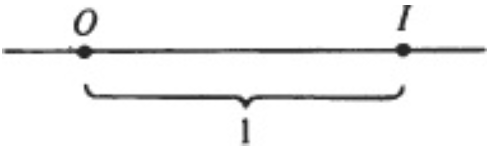
\includegraphics[width=0.3\textwidth]{pinter/assets/ch30-a-1.png}\par}

the interval $OI$ coincides with the unit interval on the $x$ axis. Let $\D$ be the set of real numbers such that $a\in\D$ if and only if the point $(a,0)$ is constructible from $\{O,I\}$. Prove the following
\begin{enumerate}
    \item If $a,b\in\D$, then $a+b\in\D$ and $a-b\in\D$.
    \item If $a,b\in\D$, then $ab\in\D$. (Hint: Use similar triangles. See the accompanying figure).
    
    {\centering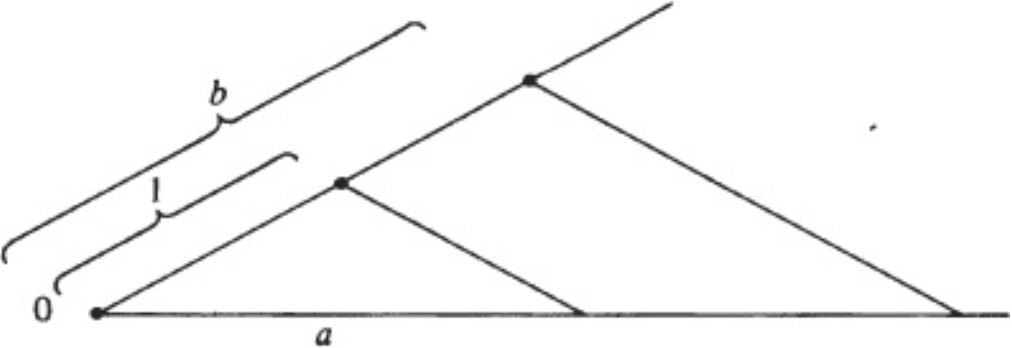
\includegraphics[width=0.5\textwidth]{pinter/assets/ch30-a-2.png}\par}
    \item If $a,b\in\D$, then $a/b\in\D$. (Use the same figure as in part 2).
    \item If $a>0$ and $a\in\D$, then $\sqrt{a}\in\D$. (Hint: In the accompanying figure, $AB$ is the diameter of a circle. Use an elementary property of chords of a circle to show that $x=\sqrt{a}$).
    
    {\centering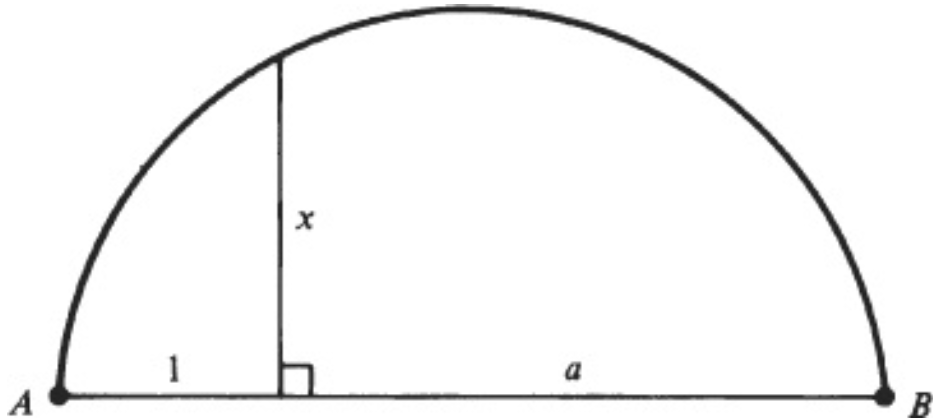
\includegraphics[width=0.5\textwidth]{pinter/assets/ch30-a-3.png}\par}

    It follows from parts 1 to 4 that $\D$ is a field, closed with respect to taking square roots of positive numbers. $\D$ is called the field of constructible numbers.
    \item $\Q\subset\D$.
    \item If $a$ is a real root of any quadratic polynomial with coefficients in $\D$, then $a\in\D$. (Hint: Complete the square and use part 4).
\end{enumerate}
\end{exercise}
\begin{proof}
 \begin{enumerate}
     \item Construct a circle around $A$ with radius $OB$. Without loss of generality, suppose $\lvert a\rvert>\lvert b\rvert$. If both $a$ and $b$ are positive, then take the furthest (from $O$) intersection of the circle with the $x$-axis. If $a$ is positive and $b$ is negative then take the closest intersection. Finally, if $a$ and $b$ are both negative, then take the furthermost point of the intersection. This gives us $a+b$. We can derive $a-b$ by using the same strategy but exchanging furthest for closest.
     \item
     \item
     \item 
     \item We have that $1\in\D$, since $a+b\in\D$, then all naturals are in $\D$. Furthermore, since all $a-b\in\D$ all integers are in $\D$. We can take this further by noticing that all quotients are in $\D$. Since $\Q$ are the quotients of all integers, then $\Q\in\D$. 
     \item
 \end{enumerate}
\end{proof}

\begin{exercise}{B Constructible points and constructible numbers}
Prove each of the following
\begin{enumerate}
    \item Let $\AAA$ be any set of points in the plane; $(a,b)$ is constructible from $\AAA$ if and only if $(a,0)$ and $(0,b)$ are constructible from  $\AAA$.
    \item If a point $P$ is constructible from $\{O,I\}$ [that is, from $(0,0)$ and $(1,0)$], then $P$ is constructible from $\Q\times\Q$.
    \item Every point in $\Q\times\Q$ is constructible from $\{O,I\}$. (Use ex.A.5. and the definition of $\D$).
    \item If a point $P$ is constructible from $\Q\times\Q$, it is constructible from $\{O,I\}$.

    By combining parts 2 and 4, we get the following important fact: Any point $P$ is constructible from $\Q\times\Q$ if and only if $P$ is constructible from $\{O,I\}$. Thus, we may define a point to be constructible if and only if it is constructible from $\{O,I\}$.
     \item A point $P$ is constructible if and only if both its coordinates are constructible numbers.
\end{enumerate}
\end{exercise}
\begin{proof}
 \begin{enumerate}
     \item 
     \item
     \item
     \item 
     \item
 \end{enumerate}
\end{proof}

\begin{exercise}{C Constructible angles}
An angle $\alpha$ is called constructible if and only if there exist constructible points $A,B$ and $C$ such that $\angle ABC=\alpha$. Prove the following:
\begin{enumerate}
    \item The angle $\alpha$ is constructible if and only if $\sin\alpha$ and $\cos\alpha$ are constructible numbers.
    \item $\cos\alpha\in\D$ if and only if $\sin\alpha\in\D$.
    \item If $\cos\alpha,\cos\beta\in\D$, then $\cos(\alpha+\beta),\cos(\alpha-\beta)\in\D$.
     \item $\cos(2\alpha)\in\D$ if and only if $\cos\alpha\in\D$.
     \item If $\alpha$ and $\beta$ are constructible angles, so are $\alpha+\beta,\alpha-\beta,(1/2)\alpha$ and $n\alpha$ for any positive integer $n$.
     \item The following angles are constructible: 30\degree, 75\degree, 22(1/2)\degree.
     \item The following angles are not constructible: 20\degree, 40\degree, 140\degree. (Hint: Use the proof of Theorem 3).
\end{enumerate}
\end{exercise}
\begin{proof}
 \begin{enumerate}
     \item 
    \item
    \item 
     \item
     \item
     \item 
     \item
 \end{enumerate}
\end{proof}

\begin{exercise}{D Constructible polygons}
A polygon is called constructible if and only if its vertices are constructible points. Prove the following:
\begin{enumerate}
    \item The regular $n$-gon is constructible if and only if the angle $2\pi/n$ is constructible. 
    \item The regular hexagon is constructible.
    \item The regular polygon of nine sides is not constructible.
\end{enumerate}
\end{exercise}
\begin{proof}
 \begin{enumerate}
     \item 
     \item
     \item
 \end{enumerate}
\end{proof}

\begin{exercise}{G Further properties of constructible numbers and figures}
Prove each of the following
\begin{enumerate}
    \item If the number $a$ is a root of an irreducible polynomial $p(x)\in\Q[x]$ whose degree is not a power of 2, then $a$ is not a constructible number.  
    \item Any constructible number can be obtained from rational numbers by repeated addition subtraction, multiplication, division, and taking square roots of positive numbers.
    \item $\D$ is the smallest field extension of $\Q$ closed with respect to square roots of positive numbers (that is, any field extension of $\Q$ closed with respect to square roots contains $\D$). (Use part 2 and exercise A).
    \item All the roots of the polynomial $x^4-3x^2+1$ are constructible numbers.

    A line is called constructible if it passes through two constructible points. A circle is called constructible if its center and radius are constructible.
    \item The line $ax+by+c=0$ is constructible if $a,b,c\in\D$.
    \item The circle $x^2+y^2+ax+by+c=0$ is constructible if $a,b,c\in\D$.
\end{enumerate}
\end{exercise}
\begin{proof}
 \begin{enumerate}
     \item 
     \item 
    \item
    \item 
    \item Suppose $a,b,c\in\D$. We have that $y=-(a/b)x-(c/b)$.
    \item
 \end{enumerate}
\end{proof}